\RequirePackage{currfile}
\documentclass[12pt]{beamer}
\usepackage[utf8]{inputenc}
\usepackage[spanish]{babel}
\usepackage{standalone}
\usepackage{color}
\usepackage{siunitx}
\usepackage{hyperref}
\usepackage[outdir=./]{epstopdf}
%\hypersetup{colorlinks,linkcolor=,urlcolor=blue}
%\hypersetup{colorlinks,urlcolor=blue}
\usepackage{xcolor,soul}
\usepackage{etoolbox}
\usepackage{amsmath}
\usepackage{amsthm}
\usepackage{mathtools}
\usepackage{tcolorbox}
\usepackage{physics}
\usepackage{multicol}
\usepackage{bookmark}
\usepackage{longtable}
\usepackage{listings}
\usepackage{cancel}
\usepackage{wrapfig}
\usepackage{empheq}
\usepackage{graphicx}
\usepackage{tikz}
\usetikzlibrary{calc, patterns, matrix, backgrounds, decorations,shapes, arrows.meta}
\usepackage[autostyle,spanish=mexican]{csquotes}
\usepackage[os=win]{menukeys}
\usepackage{pifont}
\usepackage{pbox}
\usepackage{bm}
\usepackage{caption}
\captionsetup{font=scriptsize,labelfont=scriptsize}
%\usepackage[sfdefault]{roboto}  %% Option 'sfdefault' only if the base font of the document is to be sans serif

%Sección de definición de colores
\definecolor{ao}{rgb}{0.0, 0.5, 0.0}
\definecolor{bisque}{rgb}{1.0, 0.89, 0.77}
\definecolor{amber}{rgb}{1.0, 0.75, 0.0}
\definecolor{armygreen}{rgb}{0.29, 0.33, 0.13}
\definecolor{alizarin}{rgb}{0.82, 0.1, 0.26}
\definecolor{cadetblue}{rgb}{0.37, 0.62, 0.63}
\definecolor{deepblue}{rgb}{0,0,0.5}
\definecolor{brown}{rgb}{0.59, 0.29, 0.0}
\definecolor{OliveGreen}{rgb}{0,0.25,0}
\definecolor{mycolor}{rgb}{0.122, 0.435, 0.698}

\newcommand*{\boxcolor}{orange}
\makeatletter
\newcommand{\boxedcolor}[1]{\textcolor{\boxcolor}{%
\tikz[baseline={([yshift=-1ex]current bounding box.center)}] \node [rectangle, minimum width=1ex, thick, rounded corners,draw] {\normalcolor\m@th$\displaystyle#1$};}}
 \makeatother

\newtcbox{\mybox}{on line,
  colframe=mycolor,colback=mycolor!10!white,
  boxrule=0.5pt,arc=4pt,boxsep=0pt,left=6pt,right=6pt,top=6pt,bottom=6pt}

\usefonttheme[onlymath]{serif}
%Sección de definición de nuevos comandos

\newcommand*{\TitleParbox}[1]{\parbox[c]{1.75cm}{\raggedright #1}}%
\newcommand{\python}{\texttt{python}}
\newcommand{\textoazul}[1]{\textcolor{blue}{#1}}
\newcommand{\azulfuerte}[1]{\textcolor{blue}{\textbf{#1}}}
\newcommand{\funcionazul}[1]{\textcolor{blue}{\textbf{\texttt{#1}}}}
\newcommand{\ptilde}[1]{\ensuremath{{#1}^{\prime}}}
\newcommand{\stilde}[1]{\ensuremath{{#1}^{\prime \prime}}}
\newcommand{\ttilde}[1]{\ensuremath{{#1}^{\prime \prime \prime}}}
\newcommand{\ntilde}[2]{\ensuremath{{#1}^{(#2)}}}
\renewcommand{\arraystretch}{1.5}

\newcounter{saveenumi}
\newcommand{\seti}{\setcounter{saveenumi}{\value{enumi}}}
\newcommand{\conti}{\setcounter{enumi}{\value{saveenumi}}}
\renewcommand{\rmdefault}{cmr}% cmr = Computer Modern Roman

\linespread{1.5}

\usefonttheme{professionalfonts}
%\usefonttheme{serif}
\DeclareGraphicsExtensions{.pdf,.png,.jpg}


%Sección para el tema de beamer, con el theme, usercolortheme y sección de footers
\mode<presentation>
{
  \usetheme{CambridgeUS}
  
  %\useoutertheme{infolines}
  \useoutertheme{default}
  \usecolortheme{beaver}
  \setbeamercovered{invisible}
  % or whatever (possibly just delete it)
  \setbeamertemplate{section in toc}[sections numbered]
  \setbeamertemplate{subsection in toc}[subsections numbered]
  \setbeamertemplate{subsection in toc}{\leavevmode\leftskip=3.2em\rlap{\hskip-2em\inserttocsectionnumber.\inserttocsubsectionnumber}\inserttocsubsection\par}
  \setbeamercolor{section in toc}{fg=blue}
  \setbeamercolor{subsection in toc}{fg=blue}
  \setbeamercolor{frametitle}{fg=blue}
  \setbeamertemplate{caption}[numbered]

  \setbeamertemplate{footline}
  \beamertemplatenavigationsymbolsempty
  \setbeamertemplate{headline}{}
}

\makeatletter
\setbeamercolor{section in foot}{bg=gray!30, fg=black!90!orange}
\setbeamercolor{subsection in foot}{bg=blue!30!yellow, fg=red}
\setbeamertemplate{footline}
{
  \leavevmode%
  \hbox{%
  \begin{beamercolorbox}[wd=.333333\paperwidth,ht=2.25ex,dp=1ex,center]{section in foot}%
    \usebeamerfont{section in foot} \insertsection
  \end{beamercolorbox}}%
  \begin{beamercolorbox}[wd=.333333\paperwidth,ht=2.25ex,dp=1ex,center]{subsection in foot}%
    \usebeamerfont{subsection in foot}  \insertsubsection
  \end{beamercolorbox}%
  \begin{beamercolorbox}[wd=.333333\paperwidth,ht=2.25ex,dp=1ex,right]{date in head/foot}%
    \usebeamerfont{date in head/foot} \insertshortdate{} \hspace*{2em}
    \insertframenumber{} / \inserttotalframenumber \hspace*{2ex} 
  \end{beamercolorbox}}%
  \vskip0pt%
\makeatother  

\makeatletter
\patchcmd{\beamer@sectionintoc}
  {\vfill}
  {\vskip\itemsep}
  {}
  {}
\makeatother


\title{\large{Ejercicios Segunda solución}}
\subtitle{Tema 2 - Primeras técnicas de solución}
\author{M. en C. Gustavo Contreras Mayén}
\date{}
\institute{Facultad de Ciencias - UNAM}
\titlegraphic{
\includegraphics[width=1.75cm]{../Imagenes/escudo-facultad-ciencias}\hspace*{4.75cm}~%
   
\includegraphics[width=1.75cm]{../Imagenes/escudo-unam}
}
\setbeamertemplate{navigation symbols}{}
\begin{document}
\maketitle
\fontsize{14}{14}\selectfont
\spanishdecimal{.}
\section*{Contenido}
\frame{\tableofcontents[currentsection, hideallsubsections]}
\section{Independencia lineal}
\frame{\tableofcontents[currentsection, hideothersubsections]}
\subsection{Ejercicio 1}
\begin{frame}
\frametitle{Ejercicio 1}
Si las funciones $y_{1}$ y $y_{2}$ son soluciones linealmente independientes de
\begin{align*}
\stilde{y} + p(x) \, \ptilde{y} + q(x) \, y = 0
\end{align*}
Demuestra que $c_{1} \, y_{1}$ y $c_{2} \, y_{2}$ también son soluciones linealmente independientes, siempre que $c_{1} \neq 0$ y $c_{2} \neq 0$.
\end{frame}
\begin{frame}
\frametitle{El Wronskiano}
Revisemos el Wronskiano:
\begin{align*}
W = \mdet{
c_{1} \, y_{1} & c_{2} \, y_{2} \\ 
c_{1} \, \ptilde{y}_{1} & c_{2} \, \ptilde{y}_{2}
}
\end{align*}
Desarrollemos el determinante
\end{frame}
\begin{frame}
\frametitle{El Wronskiano}
\begin{eqnarray*}
W &=& \big[ c_{1} \, y_{1} * c_{2} \, \ptilde{y}_{2} \big] - \big[ c_{1} \, \ptilde{y}_{1} * c_{2} \, y_{2} \big] = \\[0.5em] \pause
&=& c_{1} \, c_{2} \, y_{1} \, \ptilde{y}_{2} - c_{1} \, c_{2} \ptilde{y}_{1} \, y_{2} = \\[0.5em] \pause
&=& c_{1} \, c_{2} \, \big[ y_{1} \, \ptilde{y}_{2} - \ptilde{y}_{1} \, y_{2} \big] \\[0.5em] \pause
&=& c_{1} \, c_{2} \, W(y_{1}, y_{2})
\end{eqnarray*}
\end{frame}
\begin{frame}
\frametitle{Conclusión}
Dado que $y_{1}$ y $y_{2}$ son linealmente independientes, entonces $W(y_{1}, y_{2}) \neq 0$, además de que $c_{1} \neq 0$ y $c_{2} \neq 0$, se tiene que:
\begin{align*}
W(c_{1} \, y_{1}, c_{2} \, y_{2}) = c_{1} \, c_{2} \, W(y_{1}, y_{2}) \neq 0
\end{align*}
por tanto $c_{1} \, y_{1}$ y $c_{2} \, y_{2}$ son linealmente independientes.
\end{frame}
\subsection{Ejercicio 2}
\begin{frame}
\frametitle{Ejercicio 2}
Las funciones $\sin x$, $e^{x}$ y $e^{-x}$ son linealmente independientes, ya que ninguna de ellas puede escribirse como una combinación lineal de las otras dos.
\\
\bigskip
\pause
Demuestra que el Wronskiano de las tres funciones se anula pero en puntos aislados.
\end{frame}
\begin{frame}
\frametitle{Solución}
Tenemos que desarrollar el Wronskiano de las tres funciones, y revisar en qué tipo de puntos aislados se anula el determinante.
\end{frame}
\begin{frame}
\frametitle{El Wronskiano}
\begin{align*}
W = \mdet{
\sin x & e^{x} & e^{-x} \\
\cos x & e^{x} & -e^{-x} \\
-\sin x & e^{x} & e^{-x}
}
\end{align*}
\pause
Calculamos el determinante como aprendimos en álgebra lineal.
\end{frame}
\begin{frame}
\frametitle{El Wronskiano}
\begin{align*}
W &= \sin x \, \mdet{
e^{x} & -e^{x} \\
e^{x} & e^{x} \\
} - e^{x} \mdet{
\cos x & -e^{-x} \\
-\sin x & e^{-x}
} + \\[0.5em]
&+e^{-x} \mdet{
\cos x & e^{x} \\
-\sin x & e^{x}
}
\end{align*}
\end{frame}
\begin{frame}
\frametitle{El Wronskiano}
\begin{eqnarray*}
W &=& 2 \, \sin x - e^{x} \bigg[ e^{-x} \, \cos x - e^{x} \, \sin x \bigg] \\[0.5em]
&+& e^{-x} \bigg[ e^{x} \, \cos x + e^{-x} \, \sin x \bigg] = \\[0.5em] \pause
&=& 2 \, \sin x - (\cos x -\sin x) + (\cos x + \sin x) = \\[0.5em] \pause
&=& 4 \, \sin x
\end{eqnarray*}
\end{frame}
\begin{frame}
\frametitle{Revisando los puntos aislados}
Revisamos en qué puntos el Wronskiano se anula, al tener la función $\sin x$, sabemos que se anula en los puntos que son múltiplos enteros de $\pi$, por tanto:
\\
\bigskip
\pause
El Wronsiano se anula en:
\begin{align*}
W = 0 \hspace{1.5cm} x = \pm n \, \pi, \hspace{0.5cm} n = 0, 1, 2, \ldots
\end{align*}
\end{frame}
\section{Segunda solución independiente}
\frame{\tableofcontents[currentsection, hideothersubsections]}
\subsection{Ejercicio 3 - Con integrales}
\begin{frame}
\frametitle{Ejercicio 3}
Una solución de la ecuación diferencial de Laguerre
\begin{align*}
x \, \stilde{y} + (1 - x) \, \ptilde{y} + n \, y = 0
\end{align*}
para $n = 0$ es $y_{1}(x) = 1$.
\end{frame}
\begin{frame}
\frametitle{Ejercicio 1}
Utilizando la ecuación
\begin{align*}
y_{2}(x) =  y_{1} \: (x) \int^{x} \dfrac{\exp \left[ \displaystyle - \int^{x_{2}} P(x_{1}) \: \dd{x_{1}} \right]}{[y_{1}(x_{2})]^{2}} \dd{x_{2}}
\end{align*}
desarrolla una segunda solución linealmente independiente. Exhibe explícitamente el término logarítmico de la solución.
\end{frame}
\begin{frame}
\frametitle{Solución}
Ajustamos la ED inicial para dejarla en el formato
\begin{align*}
\stilde{y} + p(x) \, \ptilde{y} + q(x) \, y = 0
\end{align*}
\pause
por tanto
\begin{align*}
\stilde{y} + \dfrac{(1 - x)}{x} \, \ptilde{y} + \dfrac{n}{x} \, y = 0
\end{align*}
\end{frame}
\begin{frame}
\frametitle{Identificando la función $p(x)$}
Por lo que en este caso
\begin{align*}
p(x) = \dfrac{(1 - x)}{x} = \dfrac{1}{x} - 1
\end{align*}
que sustituiremos junto con $y_{1}(x)$ en la expresión que nos dará la segunda solución $y_{2}(x)$.
\end{frame}
\begin{frame}
\frametitle{Sustitución}
\begin{align*}
y_{2}(x) =  (1) \, \int^{x} \dfrac{\exp \left[ \displaystyle - \int^{x_{2}} \left( \dfrac{1}{x} - 1 \right) \: \dd{x_{1}} \right]}{[(1)]^{2}} \dd{x_{2}}
\end{align*}
\pause
Resolvemos primero la integral del argumento exponencial.
\end{frame}
\begin{frame}
\frametitle{Resolviendo una integral}
La integral del argumento exponencial es:
\begin{eqnarray*}
- \int^{x} p(\ptilde{x}) \dd{\ptilde{x}} = \pause - \int^{x} \bigg[ \dfrac{1}{\ptilde{x}} - 1 \bigg] \dd{\ptilde{x}}= \pause - \ln x + x
\end{eqnarray*}
\pause
Que ahora susituimos en la segunda integral para la solución.
\end{frame}
\begin{frame}
\frametitle{Sustituyendo el valor}
Así tendremos que:
\begin{eqnarray*}
y_{2} (x) = \int \exp(- \ln x + x ) \dd{x} = \pause \int \dfrac{1}{x} \, e^{x} \dd{x}
\end{eqnarray*}
\pause
Vemos que en el integrando tenemos $1/x$, que de acuerdo a lo visto en Cálculo II, la antiderivada es $\ln x$, que es el factor logarítmico que nos piden mostrar explícitamente, pero hay que hacer un ajuste en el integrando para mantener ese factor logarítmico.
\end{frame}
\begin{frame}
\frametitle{Cambio a una serie}
La función exponencial la podemos expresar en términos de una serie de potencias:
\begin{align*}
e^{x} = \sum_{k=0}^{\infty} =  1 + x + \dfrac{x^{2}}{2!} + \dfrac{x^{3}}{3!} + \dfrac{x^{4}}{4!} + \ldots
\end{align*}
\pause
Entonces usamos esta expresión en el integrando:
\end{frame}
\begin{frame}
\frametitle{Calculando la integral}
\begin{align*}
\int \dfrac{1}{x} \, e^{x} \dd{x} = \int \dfrac{1}{x} \, \bigg[ 1 + x + \dfrac{x^{2}}{2!} + \dfrac{x^{3}}{3!} + \ldots \bigg] \dd{x}
\end{align*}
\pause
Multiplicamos los términos:
\begin{align*}
y_{2} = \int \bigg[ \dfrac{1}{x} + 1 + \dfrac{x}{2!} + \dfrac{x^{2}}{3!} + \ldots \bigg] \dd{x}
\end{align*}
Calculamos la integral de cada sumando:
\end{frame}
\begin{frame}
\frametitle{Evaluando la integral}
\begin{align*}
y_{2} =  \ln (x) + x + \dfrac{x^{2}}{2 \cdot 2!} + \dfrac{x^{3}}{3 \cdot 3!} + \ldots
\end{align*}
\pause
Simplificando los términos
\begin{align*}
y_{2} =  \ln (x) + \sum_{n=1}^{\infty} \dfrac{x^{n}}{n \cdot n!}
\end{align*}
En donde se muestra explícitamente el término logarítmico de la segunda solución linealmente independiente.
\end{frame}
\subsection{Ejercicio 4 - Con series}
\begin{frame}
\frametitle{Segunda solución en series}
Encuentra los primeros términos del desarrollo en series de potencias en torno al punto regular singular $x = 0$ de la solución general de
\begin{align*}
x^{2} \stilde{y}  - x \, \ptilde{y} + (1 - x) \, y = 0, \hspace{1cm} x > 0
\end{align*} 
\end{frame}
\begin{frame}
\frametitle{Adelantando pasos}
Se puede demostrar (trabajo moral) que ocupando el método de Fronenius la ecuación de índices es:
\begin{align*}
r^{2} - 2 \, r + 1 = 0
\end{align*}
donde las raíces son: $r_{1} = r_{2} = 1$.
\end{frame}
\begin{frame}
\frametitle{Una solución a la ED}
Con $r_{1} = 1$ se obtiene (trabajo moral) una solución en términos de una serie de potencias:
\begin{align*}
y_{1}(x) &= x + x^{2} + \dfrac{x^{3}}{4} + \dfrac{x^{4}}{36} + \dfrac{x^{5}}{576} + \ldots \\[1em]
&= \sum_{k=0}^{\infty} \dfrac{1}{(k!)^{2}} \, x^{k+1}
\end{align*}
\end{frame}
\begin{frame}
\frametitle{Segunda solución}
Ya mencionamos que para obtener una segunda solución linealmente independiente $y_{2}(x)$, con $x_{0}=0$ la segunda solución es de la forma:
\begin{align*}
y_{2} (x) = y_{1}(x) \, \ln (x) + \sum_{n=1}^{\infty} b_{n} \, x^{n+1}
\end{align*}
\end{frame}
\begin{frame}
\frametitle{Desarrollo}
Lo que debemos de hacer es determinar los coeficientes $b_{n}$, susituyendo $y_{2}(x)$ directamente en la ED inicial.
\\
\bigskip
\pause
Por lo que tendremos que diferenciar $y_{2}$ hasta en dos ocasiones, para luego sustituir en la ED.
\end{frame}
\begin{frame}
\frametitle{Desarrollo}
\begin{align*}
\ptilde{y}_{2} &= \ptilde{y}_{1} \, \ln x + x^{-1} \, y_{1} + \sum_{n=1}^{\infty} (n + 1) \, b_{n} \, x^{n} \\[1em]
\stilde{y}_{2} &= \stilde{y}_{1} \, \ln x + x^{-2} \, y_{1} + 2 \, x^{-1} \, \ptilde{y} + \sum_{n=1}^{\infty} n (n + 1) \, b_{n} \, x^{n-1}
\end{align*}
\end{frame}
\begin{frame}
\frametitle{Sustitución en la ED}
Que sustiuimos en la ED inicial:
\begin{align*}
&x^{2} \left[ \stilde{y}_{1} \, \ln x + x^{-2} \, y_{1} + 2 \, x^{-1} \, \ptilde{y}_{1} + \sum_{n=1}^{\infty} n (n + 1) \, b_{n} \, x^{n-1} \right] + \\[1em]
&- x \left[ \ptilde{y}_{1} \, \ln x + x^{-1} \, y_{1} + \sum_{n=1}^{\infty} (n + 1) \, b_{n} \, x^{n} \right] + \\[0.5em]
&+ (1 - x) \left[ y_{1} \, \ln x + \sum_{n=1}^{\infty} b_{n} \, x^{n+1} \right] = 0
\end{align*}
\end{frame}
\begin{frame}
\frametitle{Factorizando}
Factorizamos términos:
\fontsize{12}{12}\selectfont
\begin{align*}
&x^{2} \left[ \stilde{y}_{1} \, \ln x + x^{-2} \, y_{1} + 2 \, x^{-1} \, \ptilde{y} + \sum_{n=1}^{\infty} n (n + 1) \, b_{n} \, x^{n-1} \right] + \\[1em]
&- x \left[ \ptilde{y}_{1} \, \ln x + x^{-1} \, y_{1} + \sum_{n=1}^{\infty} (n + 1) \, b_{n} \, x^{n+1} \right] + \\[0.5em]
&+ (1 - x) \left[ y_{1} \, \ln x + \sum_{n=1}^{\infty} b_{n} \, x^{n+1} \right] = 0
\end{align*}
\begin{tikzpicture}[overlay]
\draw [color=red] (0.9, 3.9) rectangle (3, 5.3);
\draw [color=red] (1, 2) rectangle (3.3, 3.5);
\draw [color=red] (1, 0.3) rectangle (4.3, 1.8);
\end{tikzpicture}
\end{frame}
\begin{frame}
\frametitle{Factorizando términos}
Tenemos entonces:
\begin{align*}
\bigg[ x^{2} &\, \stilde{y}_{1} - x \, \ptilde{y}_{1} + (1 - x) \, y_{1} \bigg] \, \ln x - 2 \, y_{1} +  2 \, x \, \ptilde{y}_{1} + \\[1em]
& + \sum_{n=1}^{\infty} n (n + 1) \, b_{n} \, x^{n+1} - \sum_{n=1}^{\infty} (n + 1) \, b_{n} \, x^{n+1} + \\[1em]
&+ \sum_{n=1}^{\infty} b_{n} \, x^{n+1} - \sum_{n=1}^{\infty} b_{n} \, x^{n+2} = 0
\end{align*} 
\end{frame}
\begin{frame}
\frametitle{Observación importante}
Notemos que el factor frente a $\ln x$:
\begin{align*}
\bigg[ x^{2} &\, \stilde{y}_{1} - x \, \ptilde{y}_{1} + (1 - x) \, y_{1} \bigg]
\end{align*}
es justamente el lado izquierdo de la ED inicial con $y = y_{1}$.
\\
\bigskip
Como $y_{1}$ es solución, este factor se anula.
\end{frame}
\begin{frame}
\frametitle{Continua el desarrollo}
Con la observación anterior y haciendo un corrimiento de los índices de las sumas, podemos escribir la ecuación como:
\begin{align*}
2 \, x \, \ptilde{y}_{1} -  2 \, y_{1} + b_{1} \, x^{2} +  \sum_{k=2}^{\infty} \big( k^{2} \, b_{k} - b_{k-1} \big) \, x^{k+1} = 0
\end{align*}
\end{frame}
\begin{frame}
\frametitle{Los coeficientes}
Para identificar los coeficientes $b_{k}$ y $b_{k-1}$ de modo que podamos igualarlos a cero, debemos de sustituir $y_{1}$ en su desarrollo en serie de potencias, así como $\ptilde{y}_{1}$.
\\
\bigskip
\pause
Entonces:
\begin{eqnarray*}
y_{1}(x) &=& \sum_{k=0}^{\infty} \dfrac{1}{(k!)^{2}} \, x^{k+1}\\[0.5em] \pause
\ptilde{y}_{1} (x) &=& \sum_{k=0}^{\infty} \dfrac{(k+1) \, x^{k}}{(k!)^{2}}
\end{eqnarray*}
\end{frame}
\begin{frame}
\frametitle{Sustitución de las series en la ED}
Sustituyendo las series en la ecuación que estamos desarrollando:
\begin{align*}
&\sum_{k=0}^{\infty} \dfrac{2(k + 1) - 2}{(k!)^{2}} \, x^{k+1} + b_{1} \, x^{2} + \\[0.5em]
&+ \sum_{k=2}^{\infty} \bigg[ k^{2} \, b_{k} - b_{k-1} \bigg] \, x^{k+1} = 0
\end{align*}
\end{frame}
\begin{frame}
\frametitle{Obteniendo dos términos}
Separamos los términos $k = 0$ y $k = 1$, para luego agrupar los términos semejantes:
\begin{align*}
(2 + b_{1}) \, x^{2} + \sum_{k=2}^{\infty} \bigg[ \dfrac{2 \, k}{(k!)^2} + k^{2} \, b_{k} - b_{k-1} \bigg] \, x^{k+1} = 0
\end{align*}
\\
\bigskip
\pause
Ahora igualamos a cero los coeficientes de esta expresión.
\end{frame}
\begin{frame}
\frametitle{Obteniendo los términos}
Tenemos entonces que:
\begin{align*}
(2 + b_{1}) =& \, 0 \\[1em]
\dfrac{2 \, k}{(k!)^2} + k^{2} \, b_{k} - b_{k-1} =& \, 0
\end{align*}
\end{frame}
\begin{frame}
\frametitle{Por tanto los términos}
Por lo que los términos son:
\begin{align*}
b_{1} &= -2 \\[0.5em]
b_{k} &= \dfrac{1}{k^{2}} \left[ b_{k-1} - \dfrac{2 \, k}{(k!)^{2}} \right]
\end{align*}
\pause
Por lo que ya podemos calcular los otros dos términos que nos pide el enunciado del ejercicio, es decir, $k = 2, 3$:
\end{frame}
\begin{frame}
\frametitle{Dos términos más}
\begin{eqnarray*}
b_{2} &=& \dfrac{1}{2^{2}} [b_{1} - 1] = - \dfrac{3}{4} \\[0.5em]
b_{3} &=& \dfrac{1}{9} \left[ -\dfrac{3}{4} - \dfrac{6}{36} \right] = - \dfrac{11}{108}
\end{eqnarray*}
\pause
Por tanto, una segunda solución linealmente independiente de la ED inicial es:
\begin{align*}
y_{2}(x) = y_{1}(x) \, \ln x - 2 \, x^{2} - \dfrac{3 \, x^{3}}{4} - \dfrac{11 \, x^{4}}{108} + \ldots
\end{align*}
\end{frame}
\begin{frame}
\frametitle{Gráfica de las soluciones}
\begin{figure}
   \centering
   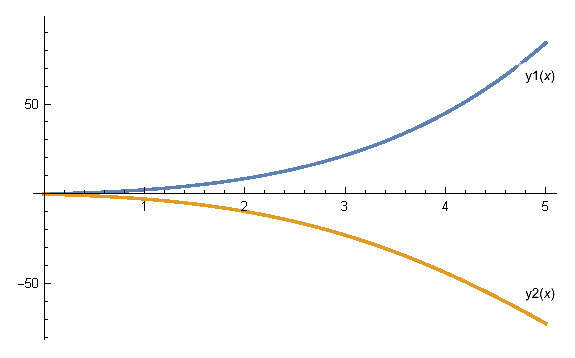
\includegraphics[scale=1]{Imagenes/Segunda_Solucion_Series_01.eps}
   \caption{Sumas parciales que aproximan las soluciones al ejercicio.}
\end{figure}
\end{frame}
\end{document}